\documentclass[tikz,border=8pt]{standalone}
\usepackage[utf8]{inputenc}
\usepackage[T1]{fontenc}
\usepackage{amsmath,amssymb}
\usetikzlibrary{arrows.meta,positioning,calc,shapes.geometric}

\definecolor{bgdark}{HTML}{0F172A}
\definecolor{paneldark}{HTML}{1E293B}
\definecolor{gridline}{HTML}{334155}
\definecolor{cellbg}{HTML}{0B1120}
\definecolor{agentblue}{HTML}{38BDF8}
\definecolor{obsred}{HTML}{EF4444}
\definecolor{freegreen}{HTML}{22C55E}
\definecolor{threatamber}{HTML}{F59E0B}
\definecolor{backpurple}{HTML}{A855F7}
\definecolor{textlight}{HTML}{F8FAFC}
\definecolor{textmuted}{HTML}{94A3B8}

% Helper macro for a 5x5 local crop (rows 1..5, cols 1..5) centered at agent (3,3)
% Local coordinates: x = col - 1 in 0..5, y = 5 - row in 0..5
% So cell (r, c) has bottom-left corner at (x = c-1, y = 5-r)
\newcommand{\drawlocalgrid}[2]{
    \fill[paneldark, rounded corners=6pt] (-1.00, -2.55) rectangle (6.60, 6.25);
    \draw[gridline, line width=0.8pt, rounded corners=6pt] (-1.00, -2.55) rectangle (6.60, 6.25);
    \node[anchor=west, text=textlight, font=\sffamily\bfseries\scriptsize] at (-0.78, 5.88) {#1};
    \node[anchor=west, text=textmuted, font=\sffamily\tiny] at (-0.78, 5.48) {#2};

    \fill[cellbg] (0, 0) rectangle (5, 5);
    \draw[gridline, line width=0.5pt] (0, 0) grid (5, 5);
    \draw[gridline, line width=0.9pt] (0, 0) rectangle (5, 5);

    % Row and col labels (rows 1..5, cols 1..5)
    \foreach \c [evaluate=\c as \x using \c-0.5] in {1,...,5} {
        \node[text=textmuted, font=\sffamily\tiny] at (\x, 5.18) {col \c};
    }
    \foreach \r [evaluate=\r as \y using 5.5-\r] in {1,...,5} {
        \node[text=textmuted, font=\sffamily\tiny] at (-0.42, \y) {fila \r};
    }
}

% Draw sensor highlight at (#1=row, #2=col, #3=color, #4=top label, #5=bottom code)
\newcommand{\drawlocalsensor}[5]{
    \pgfmathsetmacro{\sx}{#2-1}
    \pgfmathsetmacro{\sy}{5-#1}
    \fill[#3, fill opacity=0.22] (\sx+0.04, \sy+0.04) rectangle (\sx+0.96, \sy+0.96);
    \draw[#3, dashed, line width=1.0pt] (\sx+0.04, \sy+0.04) rectangle (\sx+0.96, \sy+0.96);
    \node[anchor=north, text=#3, font=\sffamily\bfseries\tiny] at (\sx+0.50, \sy+0.98) {#4};
    \node[anchor=south, text=#3, font=\ttfamily\bfseries\tiny] at (\sx+0.50, \sy+0.01) {#5};
}

% Draw obstacle at (#1=row, #2=col, #3=label)
\newcommand{\drawlocalobs}[3]{
    \pgfmathsetmacro{\ox}{#2-1}
    \pgfmathsetmacro{\oy}{5-#1}
    \fill[obsred, rounded corners=2.0pt] (\ox+0.27, \oy+0.29) rectangle (\ox+0.73, \oy+0.71);
    \node[text=white, font=\sffamily\bfseries\tiny] at (\ox+0.50, \oy+0.50) {#3};
}

% Draw agent at (3,3) facing EAST (theta=1)
\newcommand{\drawlocalagent}{
    % (r=3, c=3) -> x=2.5, y=2.5
    \begin{scope}[shift={(2.5, 2.55)}, rotate=-90]
        \fill[agentblue] (0, 0.30) -- (0.24, -0.24) -- (0, -0.12) -- (-0.24, -0.24) -- cycle;
        \draw[white, line width=0.4pt] (0, 0.30) -- (0.24, -0.24) -- (0, -0.12) -- (-0.24, -0.24) -- cycle;
    \end{scope}
    \node[anchor=south, text=agentblue, font=\sffamily\bfseries\tiny] at (2.5, 1.98) {$(3,3)$};
}

\begin{document}
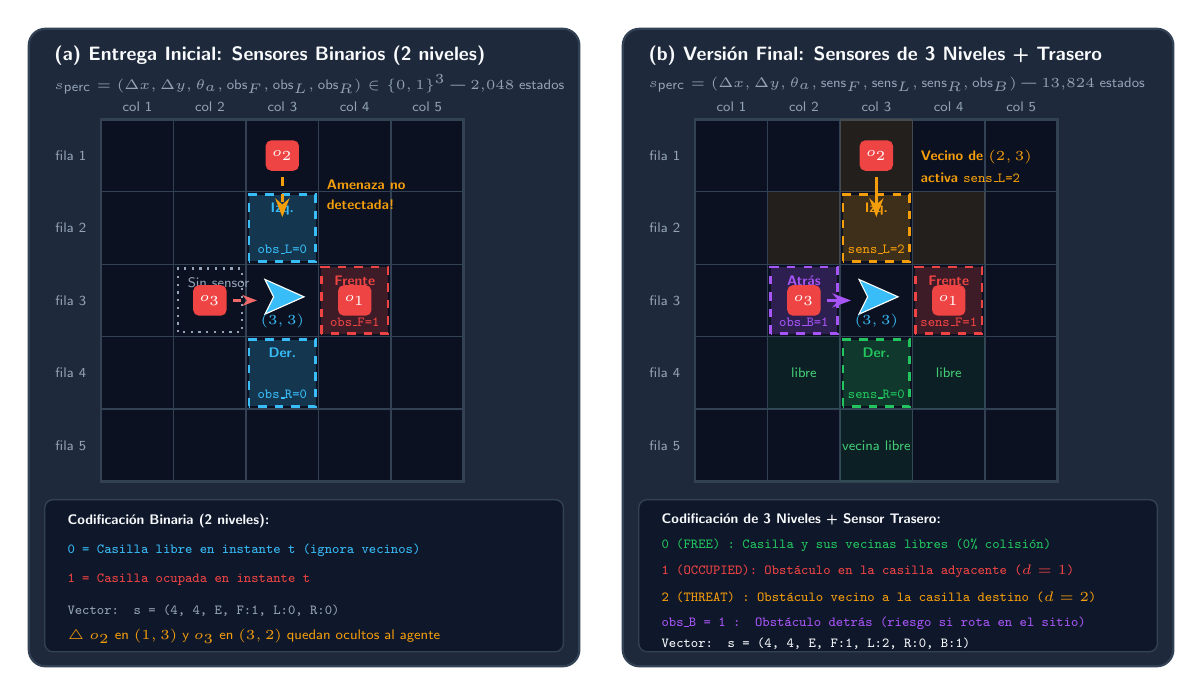
\begin{tikzpicture}[scale=0.92]

% =========================================================================
% LEFT PANEL: 2-Level Binary Sensors (Initial Delivery)
% =========================================================================
\begin{scope}[shift={(0, 0)}]
    \drawlocalgrid{(a) Entrega Inicial: Sensores Binarios (2 niveles)}{$s_{\text{perc}} = (\Delta x, \Delta y, \theta_a, \text{obs}_F, \text{obs}_L, \text{obs}_R) \in \{0,1\}^3$ --- $2{,}048$ estados}

    % Sensors around (3,3) facing EAST:
    % Front = (3,4) -> occupied (1)
    \drawlocalsensor{3}{4}{obsred}{Frente}{obs\_F=1}
    % Left = (2,3) -> binary sensor sees FREE (0) even though (1,3) has an obstacle!
    \drawlocalsensor{2}{3}{agentblue}{Izq.}{obs\_L=0}
    % Right = (4,3) -> free (0)
    \drawlocalsensor{4}{3}{agentblue}{Der.}{obs\_R=0}

    % Blind spot behind agent (3,2)
    \draw[textmuted, dotted, line width=0.8pt] (1.06, 2.06) rectangle (1.94, 2.94);
    \node[anchor=north west, text=textmuted, font=\sffamily\tiny] at (1.06, 2.94) {Sin sensor};

    % Obstacles at (3,4), (1,3), (3,2)
    \drawlocalobs{3}{4}{$o_1$}
    \drawlocalobs{1}{3}{$o_2$}
    \drawlocalobs{3}{2}{$o_3$}

    % Unseen danger arrows from o_2=(1,3)->(2,3) and o_3=(3,2)->(3,3)
    \draw[-{Stealth[scale=0.8]}, threatamber, very thick, dashed] (2.5, 4.20) -- (2.5, 3.65);
    \node[anchor=west, text=threatamber, font=\sffamily\bfseries\tiny] at (2.98, 4.10) {Amenaza no};
    \node[anchor=west, text=threatamber, font=\sffamily\bfseries\tiny] at (2.98, 3.82) {detectada!};

    \draw[-{Stealth[scale=0.8]}, obsred!80, thick, dashed] (1.82, 2.5) -- (2.15, 2.5);

    \drawlocalagent

    % Bottom summary box
    \fill[bgdark, rounded corners=3pt] (-0.78, -2.35) rectangle (6.38, -0.25);
    \draw[gridline, line width=0.5pt, rounded corners=3pt] (-0.78, -2.35) rectangle (6.38, -0.25);
    \node[anchor=west, text=textlight, font=\sffamily\bfseries\tiny] at (-0.60, -0.55) {Codificaci\'on Binaria (2 niveles):};
    \node[anchor=west, text=agentblue, font=\ttfamily\tiny] at (-0.60, -0.95) {0 = Casilla libre en instante t (ignora vecinos)};
    \node[anchor=west, text=obsred, font=\ttfamily\tiny] at (-0.60, -1.35) {1 = Casilla ocupada en instante t};
    \node[anchor=west, text=textmuted, font=\ttfamily\tiny] at (-0.60, -1.78) {Vector: s = (4, 4, E, F:1, L:0, R:0)};
    \node[anchor=west, text=threatamber, font=\sffamily\tiny] at (-0.60, -2.14) {$\triangle$ $o_2$ en $(1,3)$ y $o_3$ en $(3,2)$ quedan ocultos al agente};
\end{scope}

% =========================================================================
% RIGHT PANEL: 3-Level Sensors + Rear Sensor (Final Implementation)
% =========================================================================
\begin{scope}[shift={(8.2, 0)}]
    \drawlocalgrid{(b) Versi\'on Final: Sensores de 3 Niveles + Trasero}{$s_{\text{perc}} = (\Delta x, \Delta y, \theta_a, \text{sens}_F, \text{sens}_L, \text{sens}_R, \text{obs}_B)$ --- $13{,}824$ estados}

    % Neighborhood check around Left=(2,3) and Right=(4,3)
    % Highlight 1-hop neighborhood of Left=(2,3): (1,3), (2,2), (2,4)
    \fill[threatamber, fill opacity=0.10] (2.0, 4.0) rectangle (3.0, 5.0);
    \fill[threatamber, fill opacity=0.10] (1.0, 3.0) rectangle (2.0, 4.0);
    \fill[threatamber, fill opacity=0.10] (3.0, 3.0) rectangle (4.0, 4.0);

    % Highlight 1-hop neighborhood of Right=(4,3): (4,2), (5,3), (4,4) all clear
    \fill[freegreen, fill opacity=0.08] (1.0, 1.0) rectangle (2.0, 2.0);
    \fill[freegreen, fill opacity=0.08] (2.0, 0.0) rectangle (3.0, 1.0);
    \fill[freegreen, fill opacity=0.08] (3.0, 1.0) rectangle (4.0, 2.0);
    \node[text=freegreen!85, font=\sffamily\tiny] at (2.5, 0.5) {vecina libre};
    \node[text=freegreen!85, font=\sffamily\tiny] at (1.5, 1.5) {libre};
    \node[text=freegreen!85, font=\sffamily\tiny] at (3.5, 1.5) {libre};

    % Sensors around (3,3) facing EAST:
    % Front = (3,4) -> SENSOR_OCCUPIED (1)
    \drawlocalsensor{3}{4}{obsred}{Frente}{sens\_F=1}
    % Left = (2,3) -> SENSOR_THREAT (2) because o_2 is at (1,3)!
    \drawlocalsensor{2}{3}{threatamber}{Izq.}{sens\_L=2}
    % Right = (4,3) -> SENSOR_FREE (0) (0% collision risk!)
    \drawlocalsensor{4}{3}{freegreen}{Der.}{sens\_R=0}
    % Back = (3,2) -> obs_B = 1
    \drawlocalsensor{3}{2}{backpurple}{Atr\'as}{obs\_B=1}

    % Obstacles at (3,4), (1,3), (3,2)
    \drawlocalobs{3}{4}{$o_1$}
    \drawlocalobs{1}{3}{$o_2$}
    \drawlocalobs{3}{2}{$o_3$}

    % Threat arrow from o_2=(1,3) -> (2,3) detected by sens_L=2
    \draw[-{Stealth[scale=0.8]}, threatamber, very thick] (2.5, 4.20) -- (2.5, 3.65);
    \node[anchor=west, text=threatamber, font=\sffamily\bfseries\tiny] at (2.98, 4.48) {Vecino de $(2,3)$};
    \node[anchor=west, text=threatamber, font=\sffamily\bfseries\tiny] at (2.98, 4.20) {activa \texttt{sens\_L=2}};

    % Threat arrow from o_3=(3,2) -> (3,3) detected by obs_B=1
    \draw[-{Stealth[scale=0.8]}, backpurple, very thick] (1.82, 2.5) -- (2.15, 2.5);

    \drawlocalagent

    % Bottom summary box
    \fill[bgdark, rounded corners=3pt] (-0.78, -2.35) rectangle (6.38, -0.25);
    \draw[gridline, line width=0.5pt, rounded corners=3pt] (-0.78, -2.35) rectangle (6.38, -0.25);
    \node[anchor=west, text=textlight, font=\sffamily\bfseries\tiny] at (-0.60, -0.52) {Codificaci\'on de 3 Niveles + Sensor Trasero:};
    \node[anchor=west, text=freegreen, font=\ttfamily\tiny] at (-0.60, -0.88) {0 (FREE)    : Casilla y sus vecinas libres (0\% colisi\'on)};
    \node[anchor=west, text=obsred, font=\ttfamily\tiny] at (-0.60, -1.24) {1 (OCCUPIED): Obst\'aculo en la casilla adyacente ($d=1$)};
    \node[anchor=west, text=threatamber, font=\ttfamily\tiny] at (-0.60, -1.60) {2 (THREAT)  : Obst\'aculo vecino a la casilla destino ($d=2$)};
    \node[anchor=west, text=backpurple, font=\ttfamily\tiny] at (-0.60, -1.96) {obs\_B = 1   : Obst\'aculo detr\'as (riesgo si rota en el sitio)};
    \node[anchor=west, text=textlight, font=\ttfamily\bfseries\tiny] at (-0.60, -2.24) {Vector: s = (4, 4, E, F:1, L:2, R:0, B:1)};
\end{scope}

\end{tikzpicture}
\end{document}
